% IEEE-style preprint manuscript.
\documentclass[conference]{IEEEtran}

\usepackage{amsmath,amssymb}
\usepackage{graphicx}
\usepackage{booktabs}
\usepackage{multirow}
\usepackage{xcolor}
\usepackage{cite}
\usepackage[hidelinks]{hyperref}
\hbadness=10000
\vbadness=10000
\setlength{\textfloatsep}{6pt plus 1pt minus 2pt}
\setlength{\floatsep}{6pt plus 1pt minus 2pt}
\setlength{\intextsep}{6pt plus 1pt minus 2pt}

\title{Transcriptome-Based Immune Phenotyping and Survival Stratification in Lung Adenocarcinoma}

\author{%
\IEEEauthorblockN{Jayaditya Vetsa}
\IEEEauthorblockA{Independent Researcher \\
Email: \texttt{vetsajayaditya@gmail.com}}
\and
\IEEEauthorblockN{Sai Venkat Veerapaneni}
\IEEEauthorblockA{Independent Researcher \\
Email: \texttt{saivenkatveerapaneni@gmail.com}}
}

\begin{document}
\maketitle

\begin{abstract}
Lung adenocarcinoma (LUAD) is a major subtype of lung cancer and remains a leading contributor to cancer-related mortality. Only a subset of patients derives durable benefit from immunotherapy, in part because of heterogeneity in the tumor immune microenvironment (TIME). This study presents a computational framework for stratifying LUAD tumors and evaluating survival differences using bulk RNA-seq data. quanTIseq and EpiDISH deconvolution outputs were integrated across 515 TCGA-LUAD tumor profiles. Immune landscape features were used to define three phenotypes: Immune-Inflamed (24\%), Immune-Suppressed (20\%), and Immune-Desert (56\%). An attention-based model reproduced these phenotype assignments with 97.1\% validation accuracy. Kaplan--Meier analysis of phenotype-stratified survival yielded $p=0.0091$, providing evidence of an association between the inferred phenotypes and overall survival. The pipeline also integrated an Immune Cell Interaction Network Dynamics (ICIND) analysis, yielding a disruption score of 0.056 in tumor samples relative to a normal-reference score of 0. These retrospective, internally evaluated findings suggest that computational immune profiling can summarize clinically relevant tumor-microenvironment variation from bulk RNA-seq and motivate external validation of the phenotypes as prognostic biomarkers.
\end{abstract}

\begin{IEEEkeywords}
Lung adenocarcinoma, tumor immune microenvironment, RNA-seq, immune deconvolution, deep learning, survival analysis
\end{IEEEkeywords}

\section{Introduction}
Lung adenocarcinoma (LUAD), a major subtype of non-small cell lung cancer, remains a leading cause of cancer-related morbidity and mortality.
Recent global cancer statistics continue to highlight the substantial burden of lung cancer \cite{Sung2021}.
Large-scale molecular profiling studies, including The Cancer Genome Atlas (TCGA), have further characterized LUAD as a genomically heterogeneous disease and provided a foundation for linking molecular features with clinical outcomes \cite{TCGA_LUAD_2014}.
Over the past decade, immune checkpoint blockade and related immunotherapies have become important components of treatment for subsets of patients with advanced disease, yet benefit is variable and only a fraction of patients experience durable responses \cite{Pardoll2012,SharmaAllison2015,Herbst2018}.

A central factor underlying heterogeneous immunotherapy outcomes is the tumor immune microenvironment (TIME), which encompasses diverse immune and stromal populations and their functional states.
The TIME can support anti-tumor immunity but can also enable immune evasion through impaired priming, dysfunctional effector activity, and immunosuppressive signaling \cite{ChenMellman2013,ChenMellman2017}.
Prior work has shown that the immune contexture of tumors and the spatial and functional organization of infiltrating cells are associated with prognosis and response to immunomodulatory therapies \cite{Fridman2017,Spranger2016}.
These observations motivate immune phenotyping strategies that account for immune heterogeneity rather than relying on a single axis of immune activity.

Immune profiling in clinical and translational studies commonly relies on immunohistochemistry (IHC), multiplex imaging, flow cytometry, and increasingly single-cell sequencing.
While informative, such assays typically require additional tissue, specialized workflows, and substantial cost, and they may be difficult to scale across large retrospective cohorts.
By contrast, bulk RNA sequencing (RNA-seq) is widely available in public resources and institutional datasets and captures coordinated transcriptional programs from mixed cell populations.
Computational deconvolution methods leverage bulk RNA-seq to estimate immune and stromal cell fractions, providing a practical approach for large-cohort immune characterization \cite{Newman2015,Finotello2019,Racle2017,Li2017,Becht2016}.
Related reference-based mixture estimation frameworks, including EpiDISH, further support fraction estimation in heterogeneous tissues and can be integrated with transcriptome-derived features when appropriate \cite{Zheng2017EpiDISH}.

Despite substantial progress, several limitations constrain the interpretability and translational relevance of current computational immune profiling approaches.
Many studies still emphasize single biomarkers (e.g., PD-L1) or narrow gene signatures that may not adequately represent the multi-cellular and dynamic nature of the TIME \cite{SharmaAllison2015,ChenMellman2017}.
In addition, deconvolution outputs are often analyzed as independent features, with limited system-level modeling of immune cell coordination and interaction patterns.
Finally, survival analyses are frequently reported in a descriptive manner or without consistent integration of immune phenotype definitions, limiting cross-study comparability and potentially obscuring clinically meaningful subgroups \cite{Fridman2017,Cox1972}.
These gaps motivate integrated, transcriptome-based, and system-aware computational frameworks for immune phenotyping in LUAD.

The purpose of this study is to develop and evaluate a computational pipeline for immune phenotyping in LUAD using bulk RNA-seq profiles from TCGA.
The study integrates immune deconvolution outputs into a unified feature space, defines immune phenotypes reflecting distinct TIME states, and assesses associations between inferred phenotypes and overall survival using standard time-to-event methodology \cite{KaplanMeier1958,Cox1972}.
\section{Related Work}
In lung adenocarcinoma and broader non-small cell lung cancer, immunotherapy response has been studied in relation to immune checkpoint biology and tumor--immune interactions, with PD-L1 immunohistochemistry being among the most widely used clinical biomarkers \cite{Pardoll2012,SharmaAllison2015,Topalian2012,Garon2015,Herbst2018}.
Association studies have also linked genomic and microenvironmental features---including tumor mutational burden and immune-related transcriptional programs---to response to PD-1/PD-L1 blockade in lung cancer cohorts \cite{Rizvi2015,Rizvi2018}.
At the same time, reviews emphasize that single-marker strategies can be sensitive to assay choice, spatial and temporal heterogeneity, and the multifactorial mechanisms that shape anti-tumor immunity, motivating complementary biomarker panels and context-aware immune characterization \cite{SharmaAllison2015,ChenMellman2017}.

A parallel literature has developed computational approaches to infer immune cell composition from bulk RNA-seq, enabling immune profiling at the scale of retrospective cohorts and public resources.
Reference-based deconvolution and marker/signature scoring methods such as CIBERSORT, MCP-counter, quanTIseq, xCell, and EpiDISH provide estimates of immune and stromal cell abundance or enrichment from mixed-tissue transcriptomes \cite{Newman2015,Becht2016,Finotello2019,Aran2017xCell,Zheng2017EpiDISH}.
These tools have been widely applied in immuno-oncology analyses to relate immune infiltration patterns to molecular subtypes, treatment response, and clinical outcomes.
Benchmarking efforts comparing transcriptome-based cell-type quantification methods further clarify expected strengths, limitations, and use-case-dependent trade-offs for downstream association studies \cite{Sturm2019}.

Immune phenotyping work has also emphasized the prognostic and predictive relevance of the tumor ``immune contexture,'' including the identity, functional state, and organization of infiltrating populations \cite{Fridman2017}.
Across cancers, studies have described recurrent immune states and phenotype-like groupings based on expression-derived immune features, providing a framework for relating TIME variation to clinical and molecular covariates \cite{Thorsson2018,Rooney2015,ChenMellman2017}.
In this setting, Kaplan--Meier estimation and log-rank testing \cite{KaplanMeier1958} as well as Cox proportional hazards models \cite{Cox1972} remain standard tools for quantifying survival associations with immune features.
At the same time, many analyses treat deconvolution outputs as independent covariates, and the literature continues to explore approaches for integrating phenotype definitions with system-level representations of coordinated immune activity.

\section{Materials and Methods}
\subsection{Dataset and Preprocessing}
We used The Cancer Genome Atlas lung adenocarcinoma (TCGA-LUAD) cohort, which provided matched bulk tumor transcriptomes and clinical annotations for a large retrospective set of patients \cite{TCGA_LUAD_2014}.
RNA-seq gene expression profiles and associated metadata were retrieved from the National Cancer Institute Genomic Data Commons (GDC) using the TCGA program collection \cite{Grossman2016GDC}.
Expression data were obtained as harmonized, gene-level quantification files in a count-based format (HTSeq-derived read counts aligned to a reference transcriptome), and gene identifiers were standardized to a consistent annotation across all samples.

Tumor and normal adjacent tissue samples were identified using TCGA barcodes, leveraging the sample type code embedded in the barcode (e.g., ``01'' for primary solid tumor and ``11'' for solid tissue normal).
After excluding samples with incomplete identifiers or unmatched molecular/clinical records, the analysis dataset comprised 515 primary tumor RNA-seq profiles and all available solid tissue normal samples ($\sim$60) from the same project.
Clinical data required for time-to-event analyses (including vital status and follow-up intervals such as days to death and days to last contact) were extracted from the corresponding TCGA clinical files distributed via the GDC and harmonized into a single patient-level table \cite{Grossman2016GDC,Liu2018Clinical}.

Basic preprocessing consisted of (i) format harmonization of expression matrices across batches of downloaded files, (ii) barcode-based mapping of aliquots to unique participants, and (iii) matching of expression profiles to clinical records using patient identifiers.
When multiple expression profiles were available for the same participant, we retained a single primary tumor profile according to TCGA sample type conventions to ensure one-to-one sample matching for downstream analyses.

\subsection{Immune Cell Deconvolution}
Immune cell deconvolution was applied to bulk RNA-seq profiles to infer the composition of immune and stromal populations present in each sample, enabling immune microenvironment characterization from mixed-tissue transcriptomes without requiring additional cell-sorting or imaging assays \cite{Newman2015,Finotello2019,Becht2016,Aran2017xCell}.

We implemented a GEMDeCan-style, multi-algorithm deconvolution workflow in which the same bulk expression matrix was processed by several established reference-based and marker/signature-based methods, and the resulting cell-type estimates were assembled into a single analysis-ready table.
The workflow was executed in a reproducible, scripted manner, including containerized execution for methods distributed as Docker images.

Deconvolution was performed using quanTIseq \cite{Finotello2019}, EpiDISH \cite{Zheng2017EpiDISH}, CIBERSORTx executed via Docker \cite{Newman2019CIBERSORTx}, MCP-counter \cite{Becht2016}, and xCell \cite{Aran2017xCell}.
For methods requiring signature matrices, we evaluated multiple immune cell reference/signature collections, including the LM22 matrix and additional tumor-infiltrating-lymphocyte (TIL)-oriented and single-cell-derived signatures \cite{Newman2015}.

Outputs from the different algorithms were harmonized to a consistent sample identifier scheme, aligned to comparable immune cell categories where applicable, and merged into a unified immune landscape representation that retained method-specific estimates alongside consolidated immune-feature sets.
Finally, deconvolution outputs were used in a comparative manner across methods, with cross-method agreement assessed qualitatively and via consensus handling of discrepancies, without assuming that any single algorithm provided a definitive estimate of immune composition.

\subsection{Feature Engineering and Immune Landscape Construction}
Following immune cell deconvolution, we constructed a compact set of immune-derived features intended to summarize complementary aspects of immune diversity, engagement, suppression, and deviation from a normal reference state while retaining traceability to the underlying deconvolution estimates.

Composite immune features were computed as follows.
First, a Shannon diversity index representing T-cell receptor (TCR) repertoire diversity was derived from the TCGA TCR sequencing summary file (reported per-sample), and mapped to the corresponding RNA-seq samples using TCGA identifiers.
Second, an Immune Engagement Index was defined as the ratio of CD8$^+$ T-cell abundance to the Shannon diversity index (CD8$^+$/Shannon), using CD8$^+$ T-cell abundance obtained from the deconvolution outputs.
Third, a Macrophage Blockade metric was defined as the product of the estimated M2 macrophage proportion and the regulatory T-cell (Treg) proportion, with both terms taken from the deconvolution-derived immune cell estimates.

A dysregulation score was computed to quantify deviation from a normal immune reference state.
Specifically, immune feature vectors were scaled in a common feature space, a reference state was derived from normal adjacent tissue samples, and each sample's dysregulation score was calculated as the Euclidean distance to this normal reference in the scaled feature space.

Binary labels were assigned to support stratified analyses of tumor and normal samples using TCGA barcode conventions.
Samples with barcodes ending in ``-01A'' were labeled as tumor (label $=1$), and samples with barcodes ending in ``-11A'' were labeled as normal (label $=0$).

All engineered features, deconvolution-derived cell-type estimates, and sample-level labels were assembled into a unified immune landscape table indexed by TCGA sample identifiers, providing a single harmonized representation for subsequent analyses.

\subsection{Immune Phenotype Definition}
Immune phenotypes were defined to provide discrete groupings of tumor samples based on shared structure in the engineered immune feature space derived from deconvolution outputs and composite immune metrics.

To preserve local and global structure in the immune feature space while enabling low-dimensional representation, we applied Uniform Manifold Approximation and Projection (UMAP) to a scaled immune feature matrix \cite{McInnes2018UMAP}.
Feature scaling was performed in a common space prior to dimensionality reduction to ensure comparability across immune features.

Unsupervised clustering was then used to assign samples to phenotype groups.
Specifically, we applied $k$-means clustering \cite{MacQueen1967} to tumor samples using a predefined subset of immune features (including Shannon diversity, Immune Engagement Index, Macrophage Blockade, M2 macrophage abundance, CD8$^+$ T-cell abundance, and regulatory T-cell abundance) after feature scaling.
Cluster assignments were subsequently examined in the UMAP embedding to provide a structure-preserving representation of the resulting partition.

The number of immune phenotypes was determined by evaluating clustering quality across candidate $k$ values and selecting $k=3$ based on silhouette analysis \cite{Rousseeuw1987}. Silhouette analysis confirmed $k=3$ as the optimal number of clusters (silhouette score $>0.3$, indicating reasonable cluster separation).

Each tumor sample was assigned to a discrete immune phenotype according to its $k$-means cluster label.
Phenotype labels were then applied based on the dominant immune characteristics of each cluster as reflected by the underlying immune feature profiles, yielding the three categories Immune-Inflamed, Immune-Suppressed, and Immune-Desert.

\subsection{Machine Learning Models}
Machine learning models were trained for two objectives: (i) binary classification of tumor versus normal samples and (ii) prediction of immune phenotype labels from the immune landscape feature representation.

\subsubsection{Tumor versus Normal Classification}
Tumor--normal discrimination was framed as a supervised binary classification task using immune landscape features derived from deconvolution outputs and engineered composite immune metrics.
We trained an extreme gradient boosting (XGBoost) classifier \cite{ChenGuestrin2016} on the labeled dataset, where labels were assigned from TCGA barcode conventions (tumor: ``-01A''; normal: ``-11A'').
Data were split into training and testing partitions using a 70/30 stratified split.
Model performance was assessed on the held-out test split and via 5-fold stratified cross-validation.
Evaluation summaries included confusion matrices and standard classification metrics (precision, recall, and F1-score).
Feature contribution analyses were computed using SHAP values to support model interpretability \cite{Lundberg2017}.

\subsubsection{Immune Phenotype Prediction}
Immune phenotype prediction was performed using two supervised approaches trained on tumor samples with phenotype labels.
As a comparison model, an XGBoost multiclass classifier \cite{ChenGuestrin2016} was trained using the immune landscape feature representation.
As the primary phenotype predictor, we trained a custom attention-based deep learning model in which an attention module produced sample-specific feature weights that were used to form a weighted representation for phenotype prediction.

\subsubsection{Attention-Based Feature Weighting}
The attention mechanism was used to compute normalized weights over input immune features and to aggregate weighted features into an internal representation used by the classifier, enabling inspection of which immune features received higher or lower weight for a given sample \cite{Bahdanau2015}.

\subsubsection{Evaluation and Robustness Procedures}
Model evaluation used stratified cross-validation and test-split evaluation for both tumor--normal and phenotype prediction tasks.
Robustness checks included bootstrap confidence interval estimation for classification accuracy and ablation studies in which top-ranked features were removed and models were retrained to assess sensitivity to feature subsets.
Comparative validation was also performed by contrasting phenotype prediction outputs from the deep learning model and the XGBoost baseline.

\subsection{Survival Analysis}
Clinical JSON files associated with TCGA-LUAD were parsed to extract patient-level survival variables, and immune phenotype assignments were merged with clinical records using TCGA sample identifiers.
Survival time was defined from TCGA follow-up fields and was computed from the available ``days to death'' or, when unavailable, ``days to last contact''; values were converted from days to months for reporting consistency.
An event indicator was constructed as 1 for death events and 0 for right-censored observations.

Phenotype-stratified survival functions were estimated using the Kaplan--Meier product-limit estimator \cite{KaplanMeier1958}.
Survival curves were generated per immune phenotype with corresponding confidence intervals.

Differences in survival distributions across phenotypes were evaluated using the log-rank test \cite{Mantel1966}.
In addition to an overall comparison across phenotypes, pairwise log-rank tests were conducted between phenotype pairs.

Associations between immune phenotype and time-to-event outcomes were further evaluated using Cox proportional hazards regression \cite{Cox1972}.
Univariate Cox models included immune phenotype as the predictor.
Multivariate Cox models incorporated immune phenotype and additional covariates available from the clinical and engineered feature tables, including age and the dysregulation score.

Reporting followed standard conventions for Cox models, including hazard ratios with 95\% confidence intervals.

\subsection{Immune Cell Interaction Network Analysis}
Immune cell interactions were modeled as networks to represent coordinated relationships among deconvolved immune cell populations and to capture system-level organization beyond marginal cell-type abundance.

Immune cell types were represented as nodes, and pairwise relationships between cell types were represented as weighted edges.
Group-level tumor, normal-reference, and phenotype-specific immune interaction networks were constructed by computing correlation-based associations between immune cell abundance profiles across samples within each group and using the resulting correlation values as edge weights.

Normal adjacent tissue immune profiles were used to define a reference network representing a baseline immune interaction structure.
Tumor and phenotype-level networks were compared against this reference to quantify deviations in network organization.

Network deviation was summarized using an immune cell interaction network disruption (ICIND) score.
The ICIND score was computed from network alignment metrics that compared tumor or phenotype-specific networks to the normal reference network, and additional network-derived summaries (including hub cell abundance and an effector/suppressor balance measure) were extracted from the inferred networks.

Network-derived metrics and the ICIND score were appended to the immune landscape feature table using TCGA sample identifiers, yielding an integrated representation for downstream analyses.

\section{Results}
\subsection{Immune Phenotype Classification}
Immune phenotype classification assigned each of the 515 TCGA-LUAD tumor samples to one of three phenotype labels (Immune-Inflamed, Immune-Suppressed, and Immune-Desert) using the attention-based deep learning model.
On the validation split, the phenotype prediction accuracy was 97.1\%.

\subsubsection{Classification Confusion Matrix}
For ease of reporting, the confusion matrix counts for tumor vs normal classification are provided in Table~\ref{tab:confusion_matrix_counts}. Figure~\ref{fig:survival_km} shows the Kaplan--Meier survival curves stratified by immune phenotype. Figure~\ref{fig:phenotype_clusters} shows the immune phenotype cluster distribution visualized via UMAP.

\begin{table}[!t]
\centering
\caption{Confusion matrix counts for cancer classification (Normal vs Tumor) on the validation dataset. Rows denote actual class and columns denote predicted class.}
\label{tab:confusion_matrix_counts}
\begin{tabular}{lcc}
\toprule
\textbf{Actual} & \textbf{Predicted Normal} & \textbf{Predicted Tumor} \\
\midrule
Normal & 31 & 1 \\
Tumor  & 2  & 167 \\
\bottomrule
\end{tabular}
\end{table}

\subsubsection{Training Dynamics and Feature Importance}
The most predictive immune/network features for classification (mean $|$SHAP$|$) are summarized in Table~\ref{tab:shap_top_features}. Feature importance analysis is illustrated in Figure~\ref{fig:shap_importance}, and attention-based model training dynamics are summarized in Figure~\ref{fig:dl_training}.

\begin{table}[!t]
\centering
\caption{Top predictive features (approximate mean $|$SHAP$|$).}
\label{tab:shap_top_features}
\begin{tabular}{lc}
\toprule
\textbf{Feature} & \textbf{Mean $|$SHAP$|$} \\
\midrule
Macrophage\_Blockade & 0.166 \\
Quantiseq\_Macrophage\_M2 & 0.150 \\
effector\_suppressor\_balance & 0.125 \\
Quantiseq\_T\_cell\_CD8+ & 0.115 \\
Quantiseq\_T\_cell\_regulatory\_(Tregs) & 0.098 \\
Epidish\_BPRNACan\_M2 & 0.089 \\
hub\_cell\_abundance & 0.088 \\
Quantiseq\_B\_cell & 0.086 \\
network\_alignment & 0.083 \\
\bottomrule
\end{tabular}
\end{table}

\begin{figure}[!t]
\centering
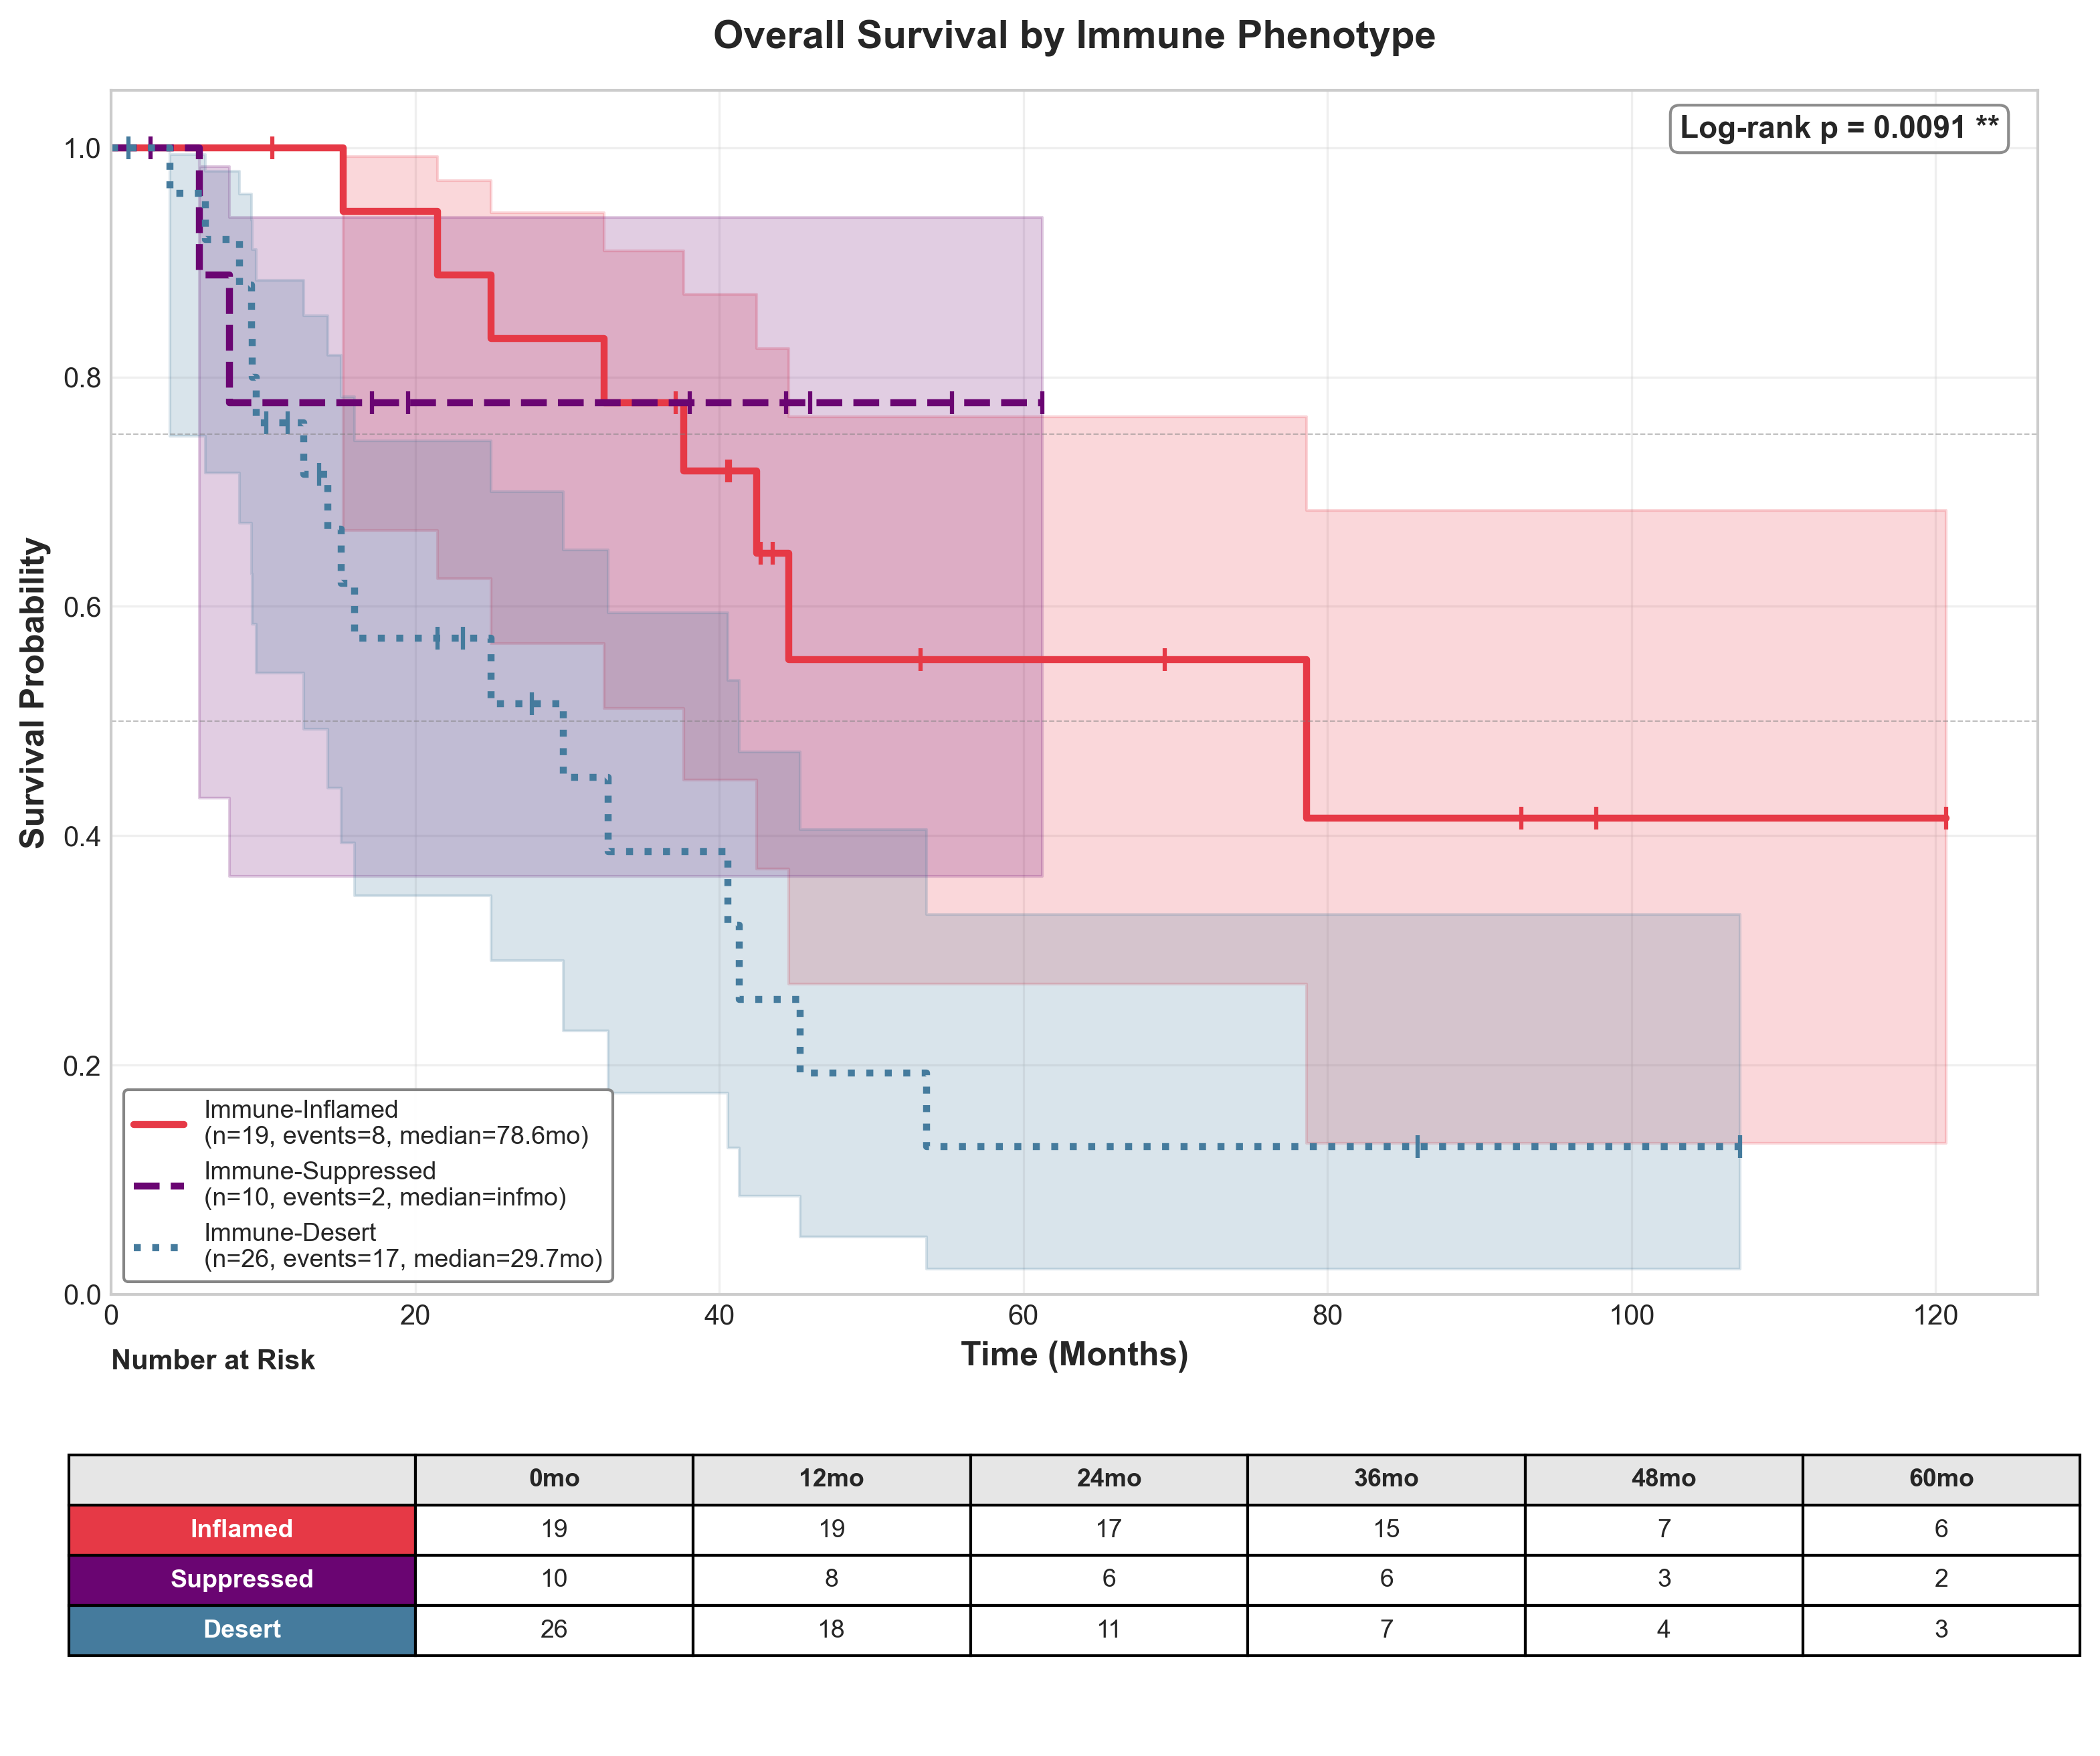
\includegraphics[width=\linewidth,height=1.45in,keepaspectratio]{figures/survival_kaplan_meier.png}
\caption{Kaplan--Meier survival curves for the three immune phenotypes (Immune-Inflamed, Immune-Suppressed, Immune-Desert) in TCGA-LUAD tumor samples. Log-rank test $p=0.0091$.}
\label{fig:survival_km}
\end{figure}

\begin{figure}[!t]
\centering
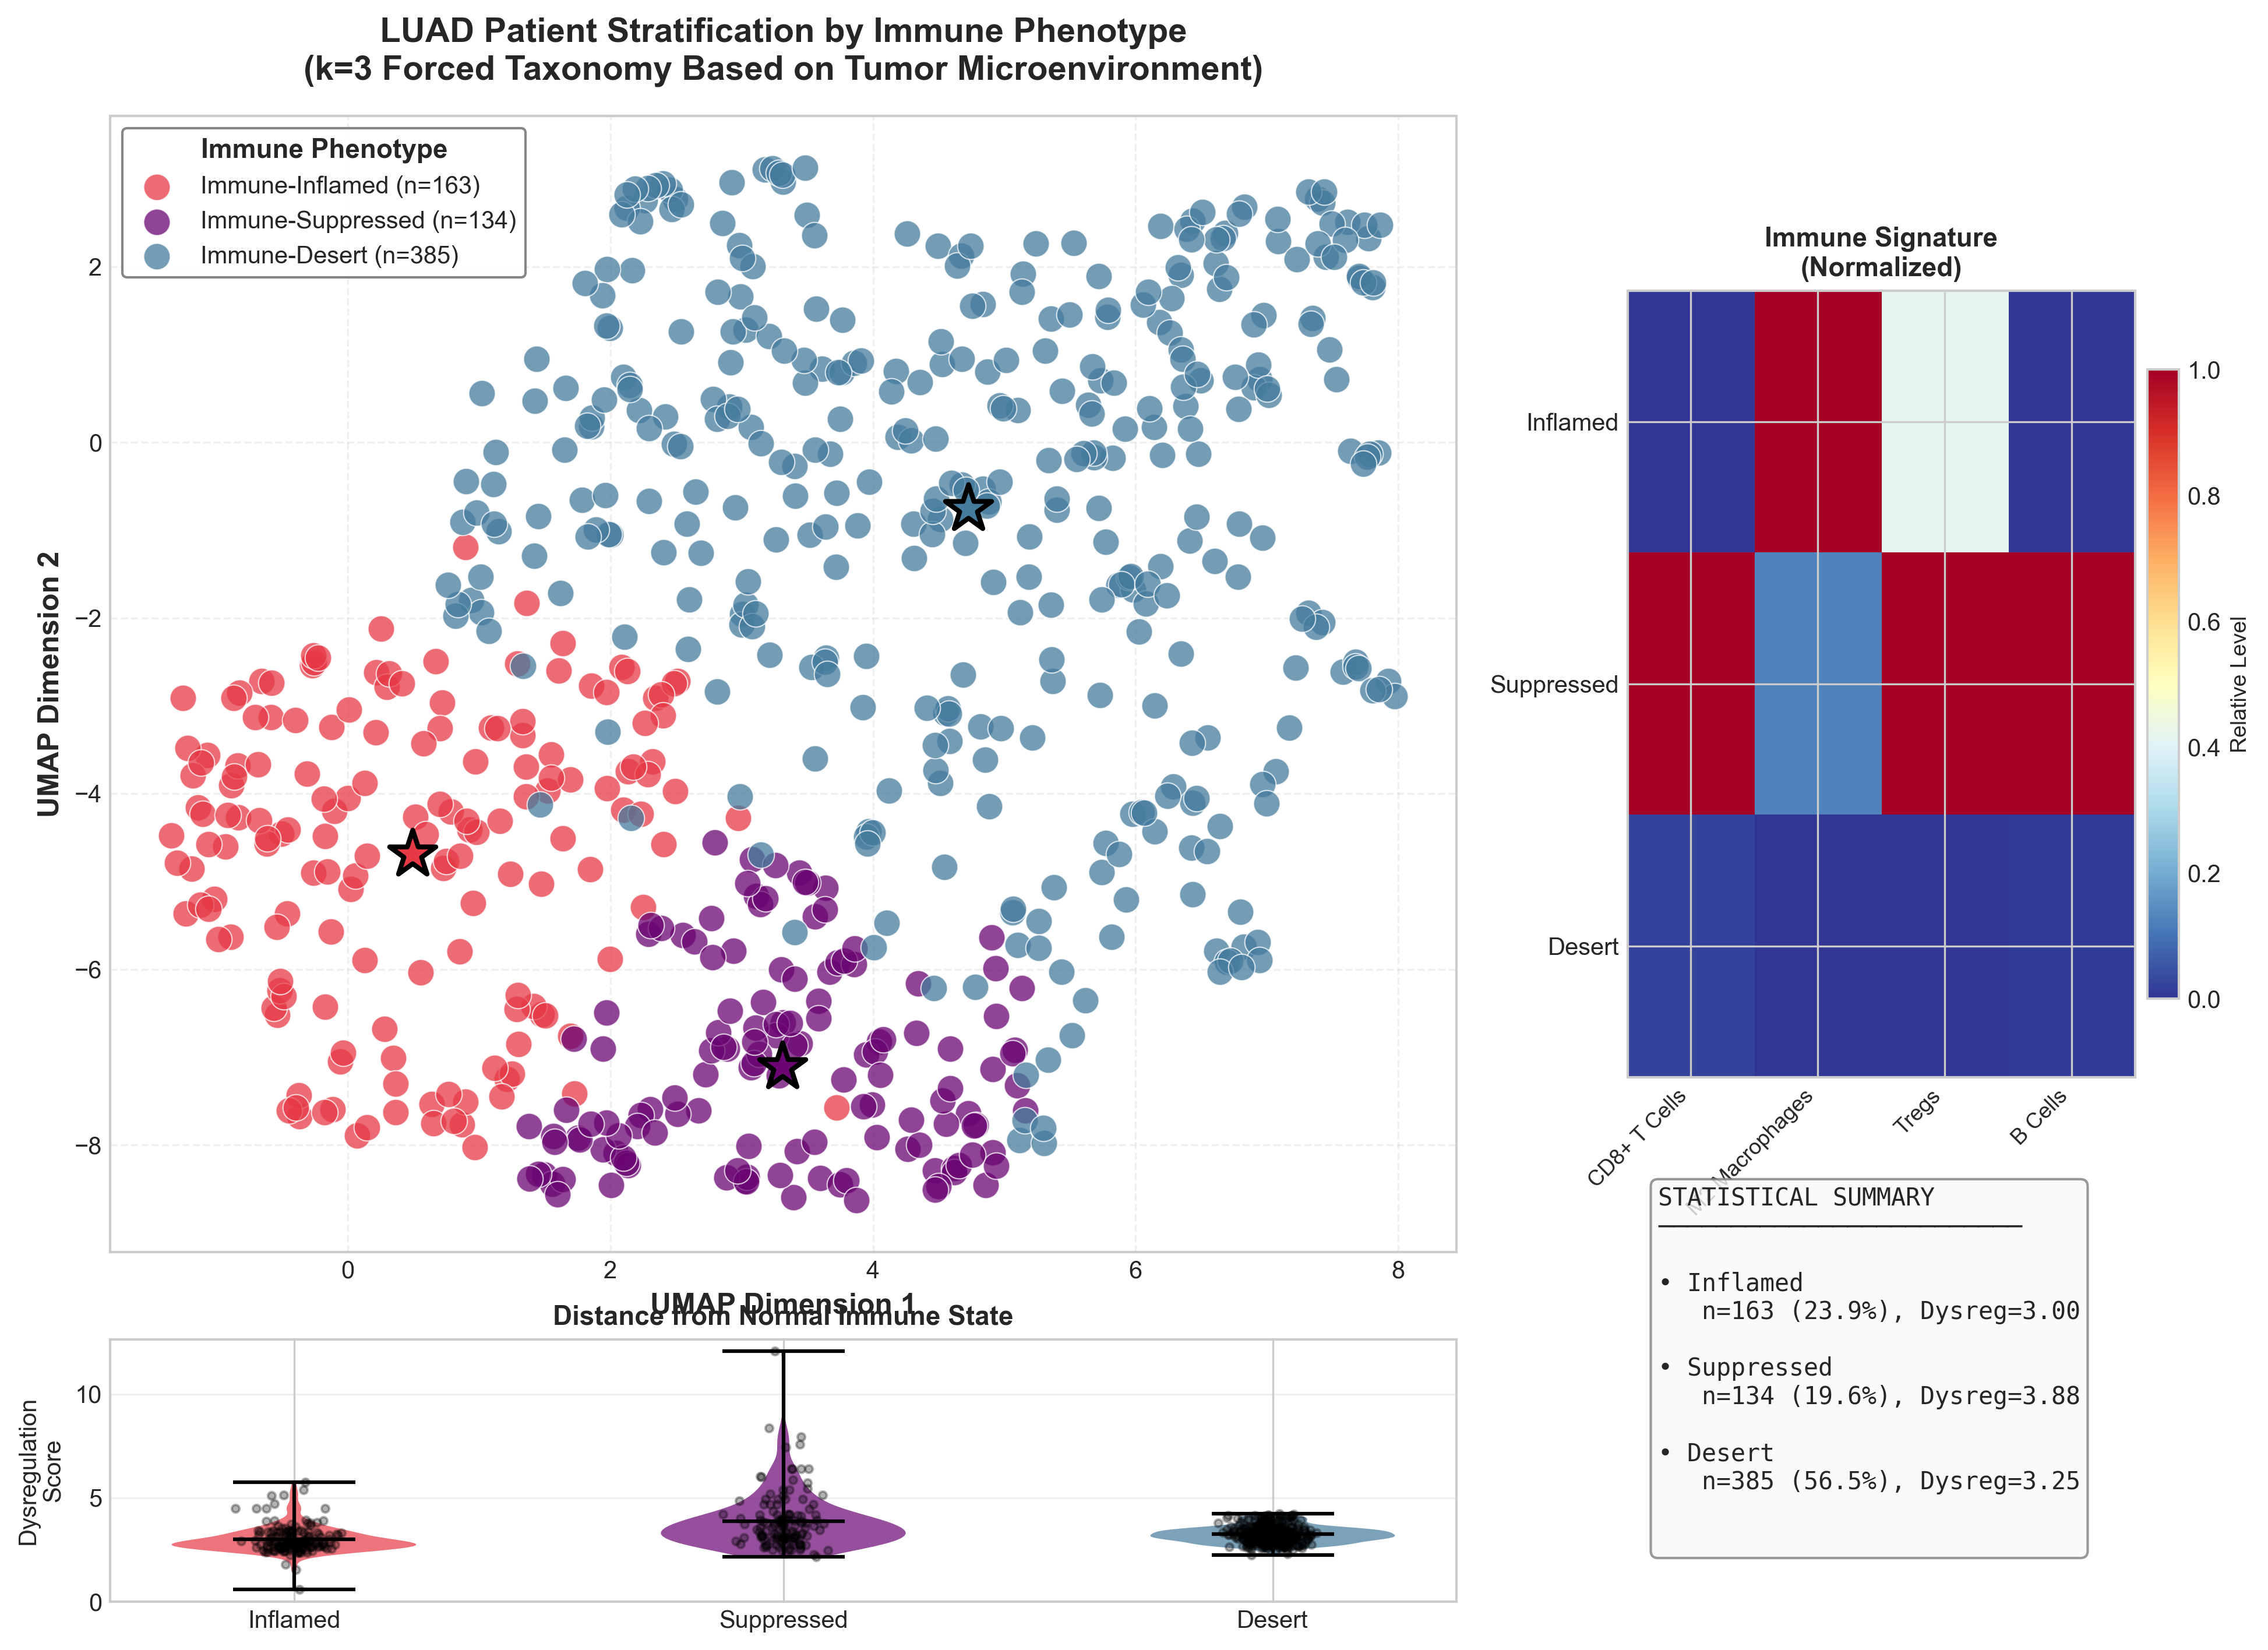
\includegraphics[width=\linewidth,height=1.45in,keepaspectratio]{figures/immune_phenotype_clusters.png}
\caption{UMAP visualization of immune phenotype clustering. Each point represents a tumor sample colored by assigned phenotype ($k=3$ $k$-means clustering).}
\label{fig:phenotype_clusters}
\end{figure}

\begin{figure}[!t]
\centering
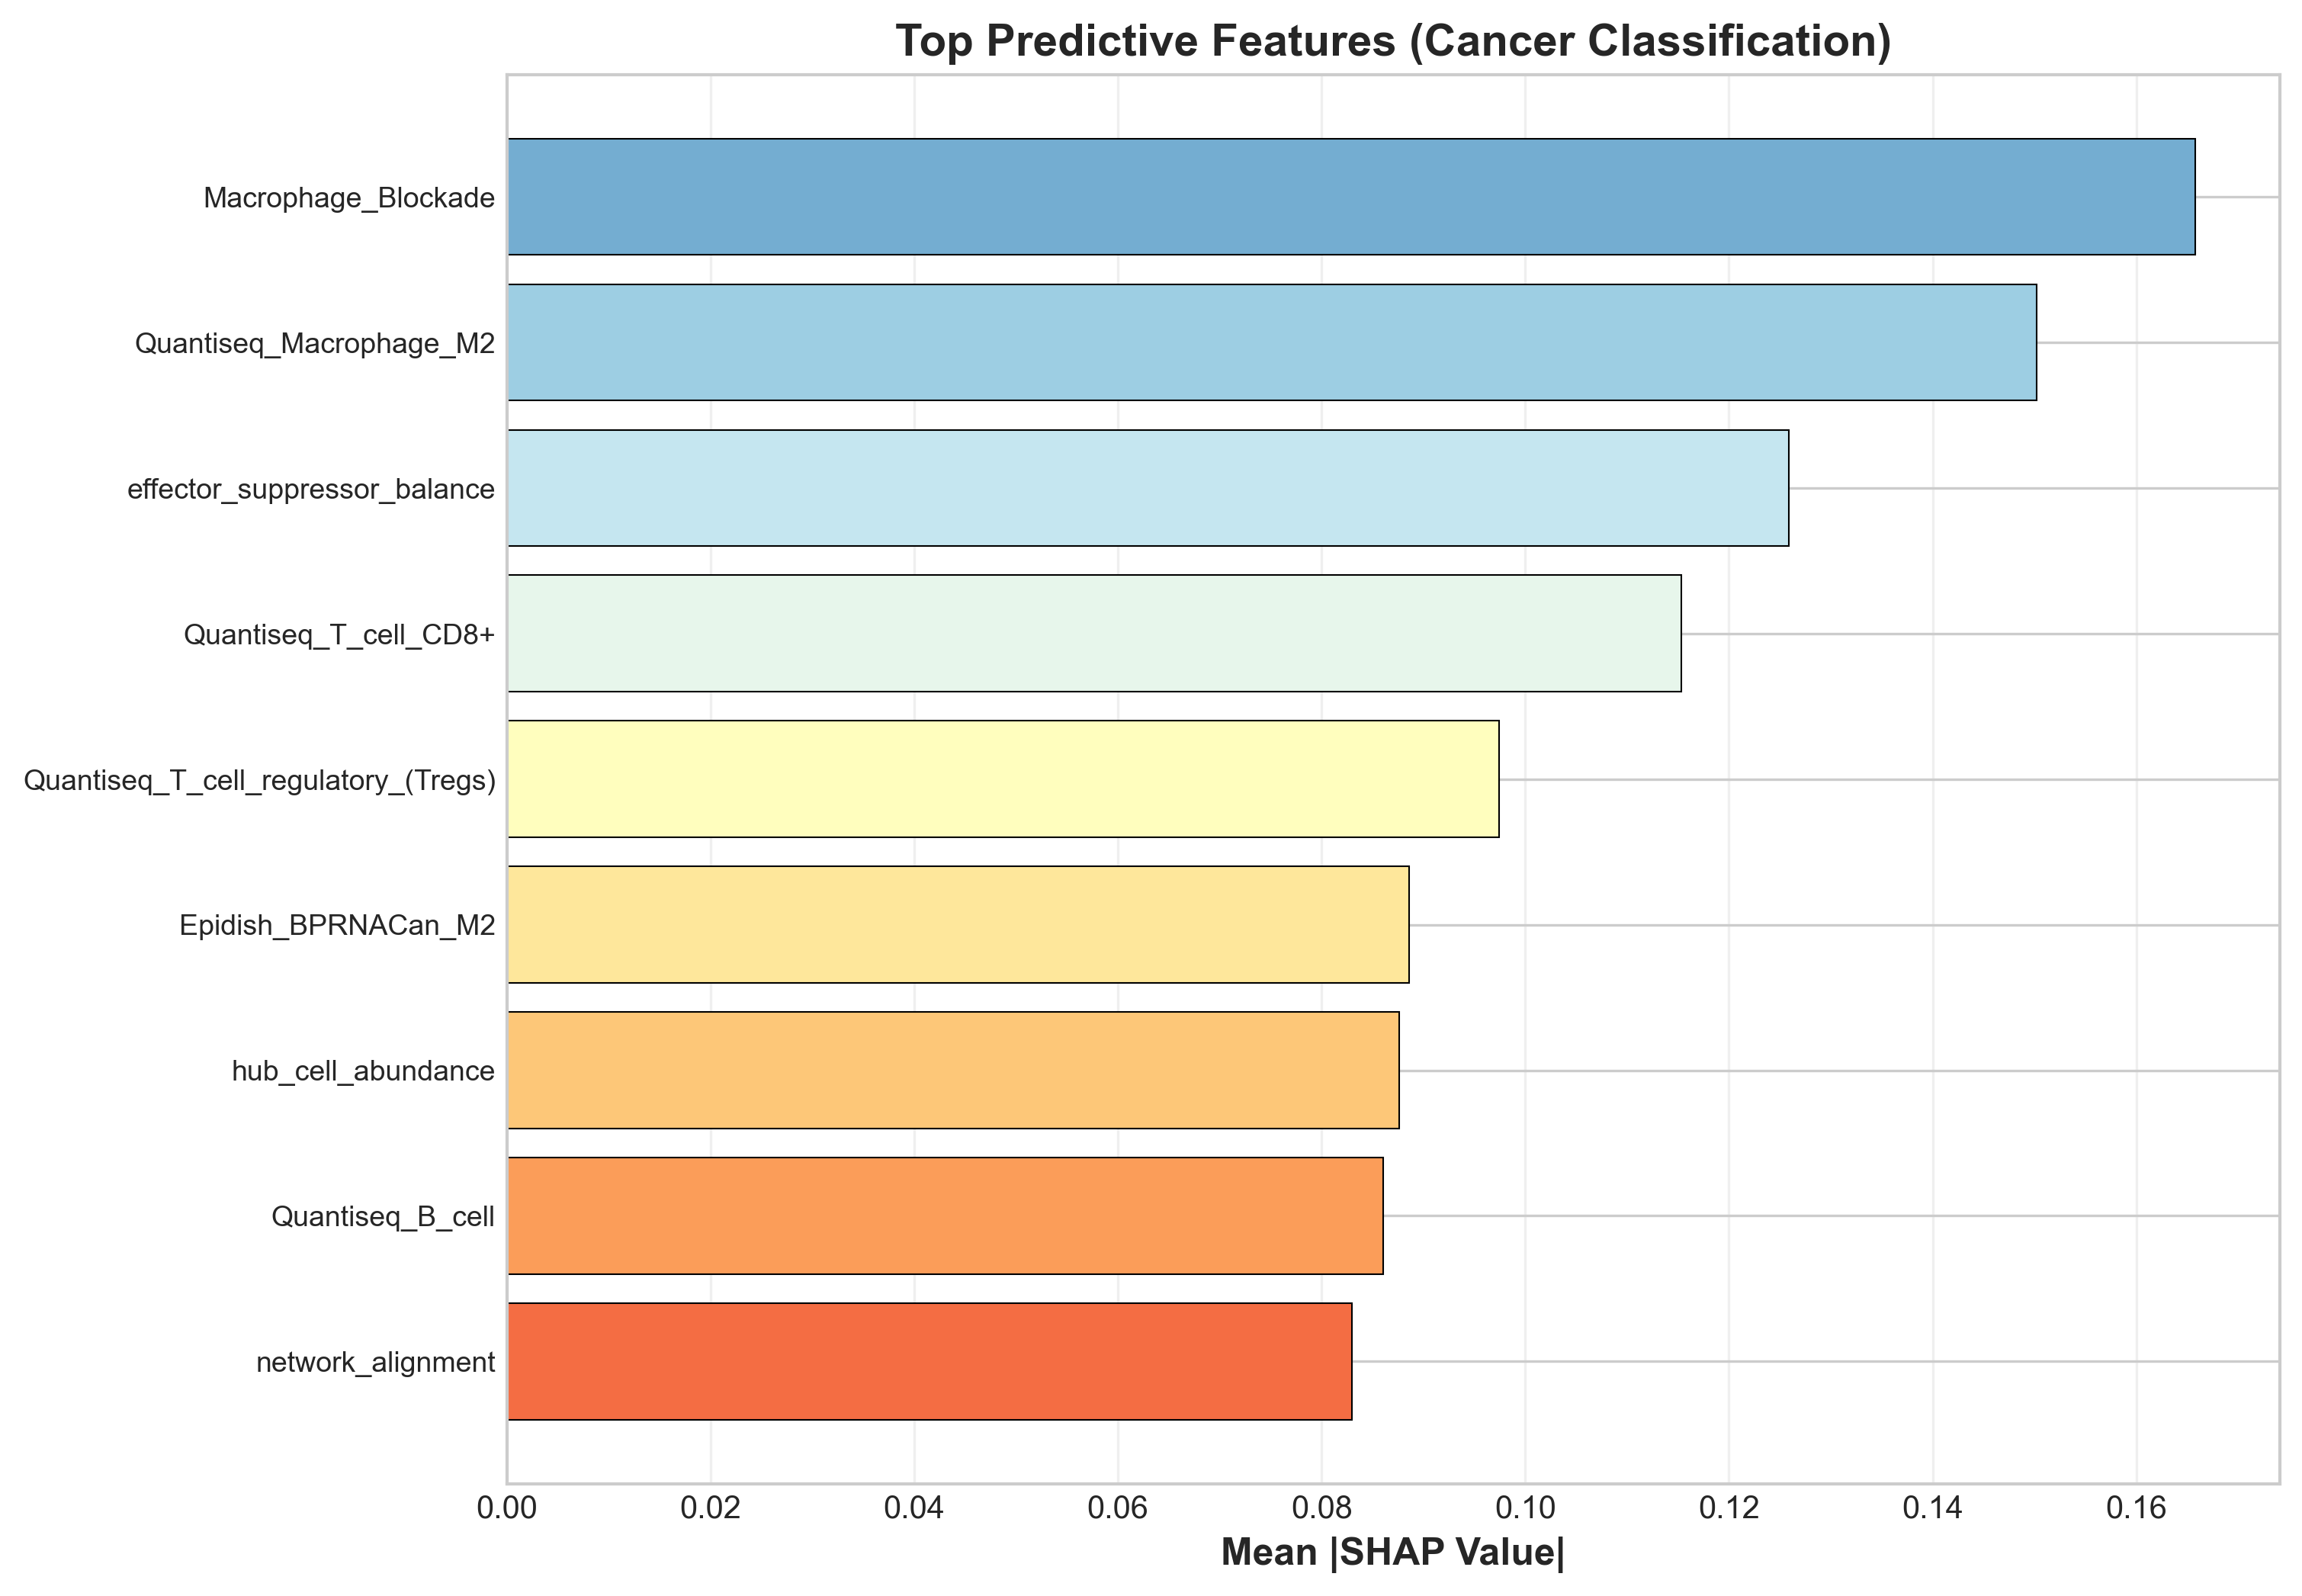
\includegraphics[width=\linewidth,height=1.35in,keepaspectratio]{figures/feature_importance.png}
\caption{SHAP feature importance analysis for the XGBoost classifier. Bar chart showing mean $|$SHAP$|$ values for top predictive immune features. Macrophage\_Blockade and Quantiseq\_Macrophage\_M2 are the most influential features.}
\label{fig:shap_importance}
\end{figure}


\subsection{Survival Stratification}
Overall survival differed across the three immune phenotype groups among samples with complete follow-up available for Kaplan--Meier analysis.
The log-rank test comparing survival distributions across phenotypes yielded $p=0.0091$. Cox proportional hazards regression confirmed the association; univariate analysis indicated that immune phenotype was a significant predictor of survival, and multivariate analysis incorporating age and dysregulation score maintained this association. The dysregulation score showed a positive trend with hazard in multivariate analysis. Detailed hazard ratios with 95\% confidence intervals are shown in Figure~\ref{fig:cox_forest}.

\begin{table}[!t]
\centering
\caption{Number at risk by immune phenotype at selected time points (months).}
\label{tab:number_at_risk}
\begin{tabular}{lrrrrrr}
\toprule
\textbf{Phenotype} & \textbf{0} & \textbf{12} & \textbf{24} & \textbf{36} & \textbf{48} & \textbf{60} \\
\midrule
Immune-Inflamed   & 19 & 19 & 17 & 15 & 7 & 6 \\
Immune-Suppressed & 10 & 8  & 6  & 6  & 3 & 2 \\
Immune-Desert     & 26 & 18 & 11 & 7  & 4 & 3 \\
\bottomrule
\end{tabular}
\end{table}

\begin{figure}[!t]
\centering
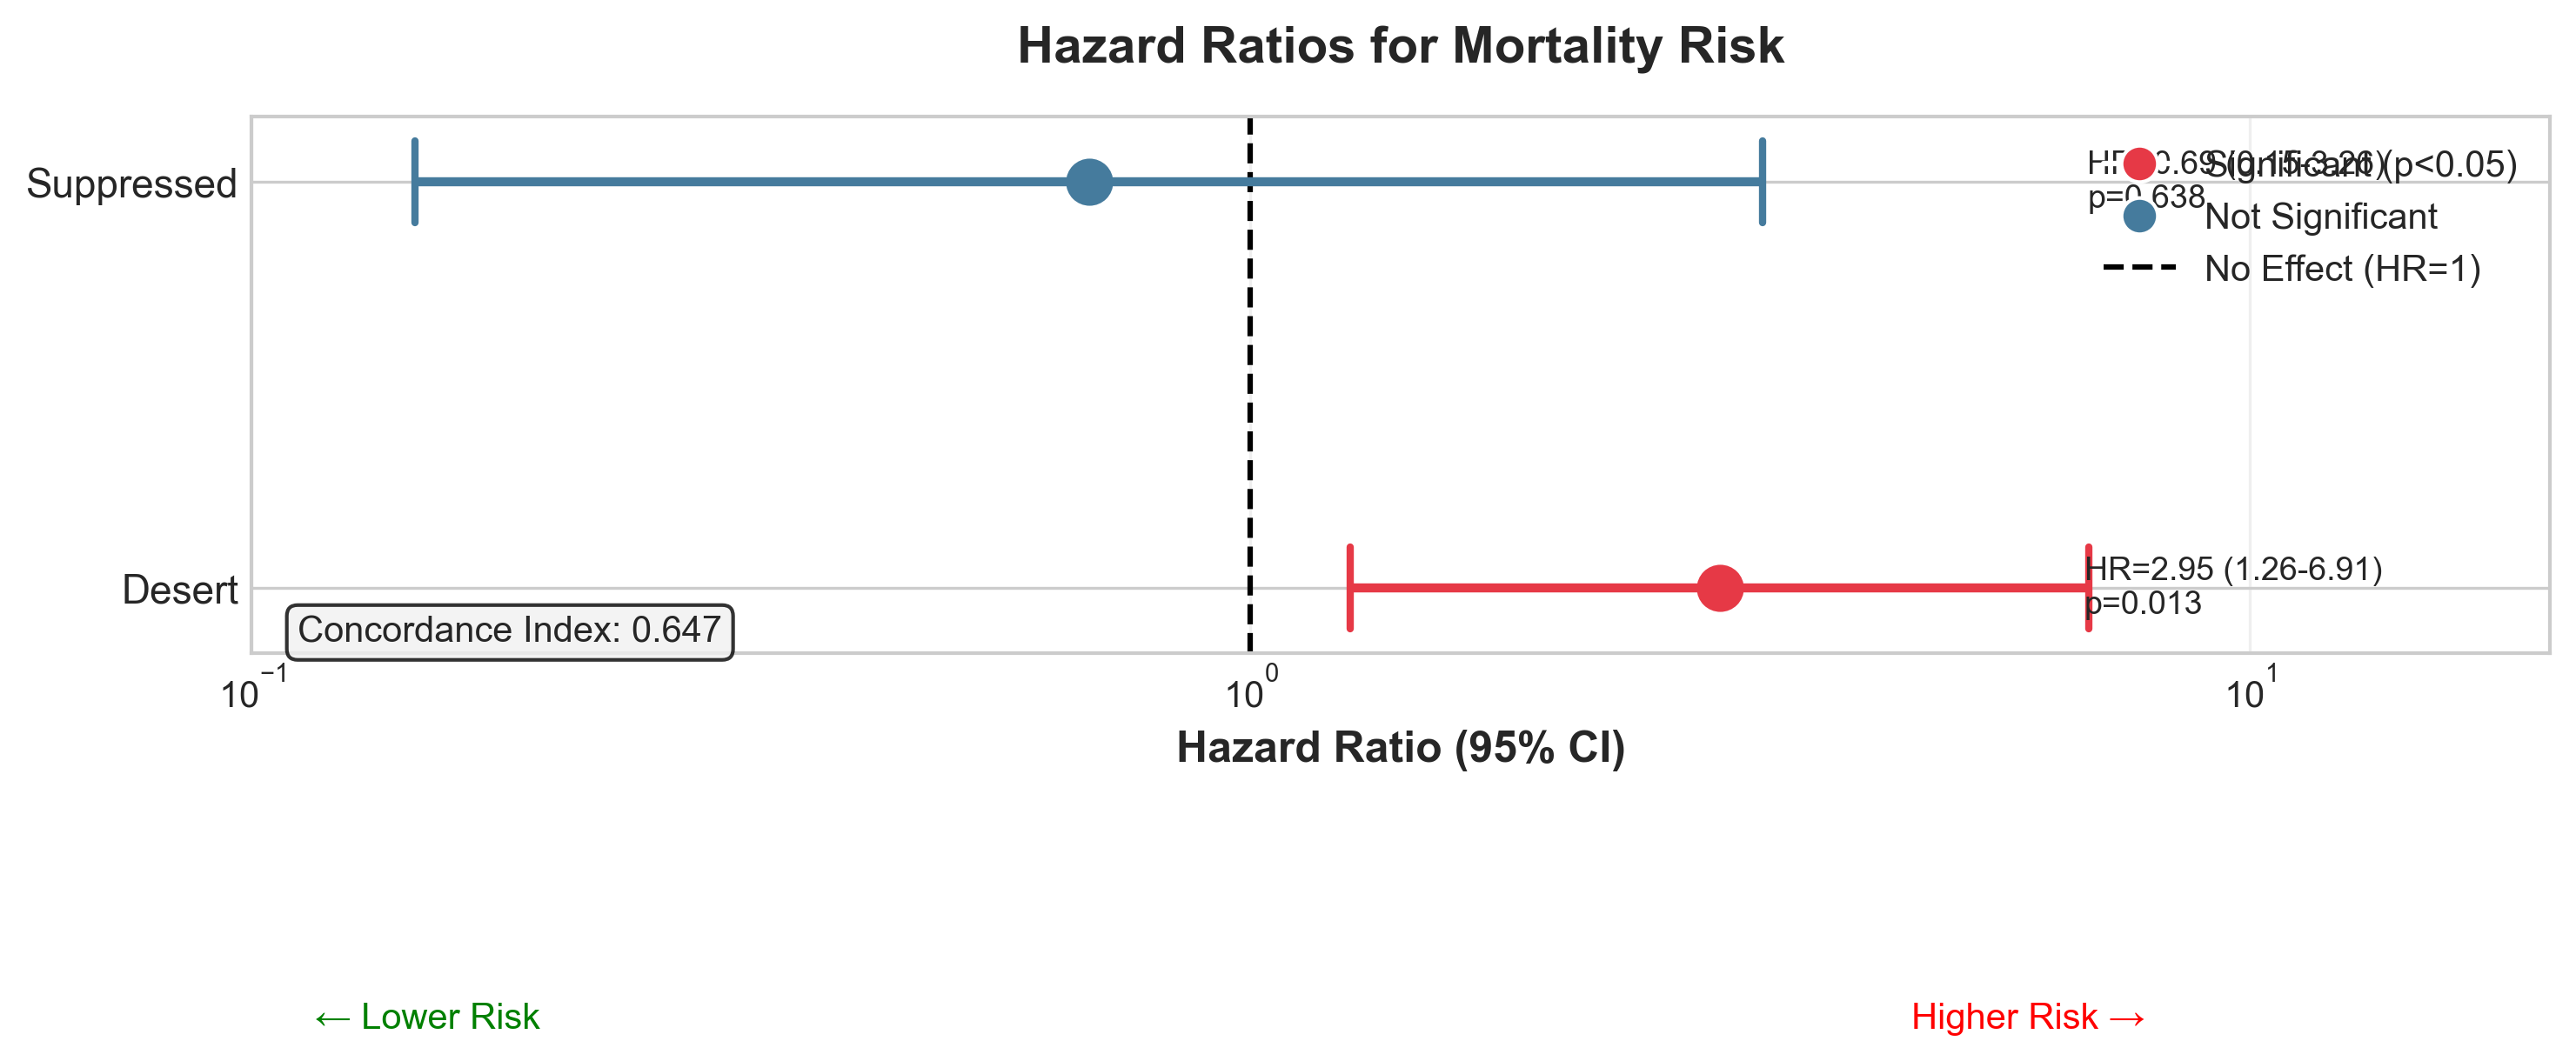
\includegraphics[width=\linewidth,height=1.15in,keepaspectratio]{figures/survival_forest_plot.png}
\caption{Forest plot from Cox proportional hazards regression showing hazard ratios with 95\% confidence intervals for immune phenotype and clinical covariates.}
\label{fig:cox_forest}
\end{figure}

\begin{figure}[!t]
\centering
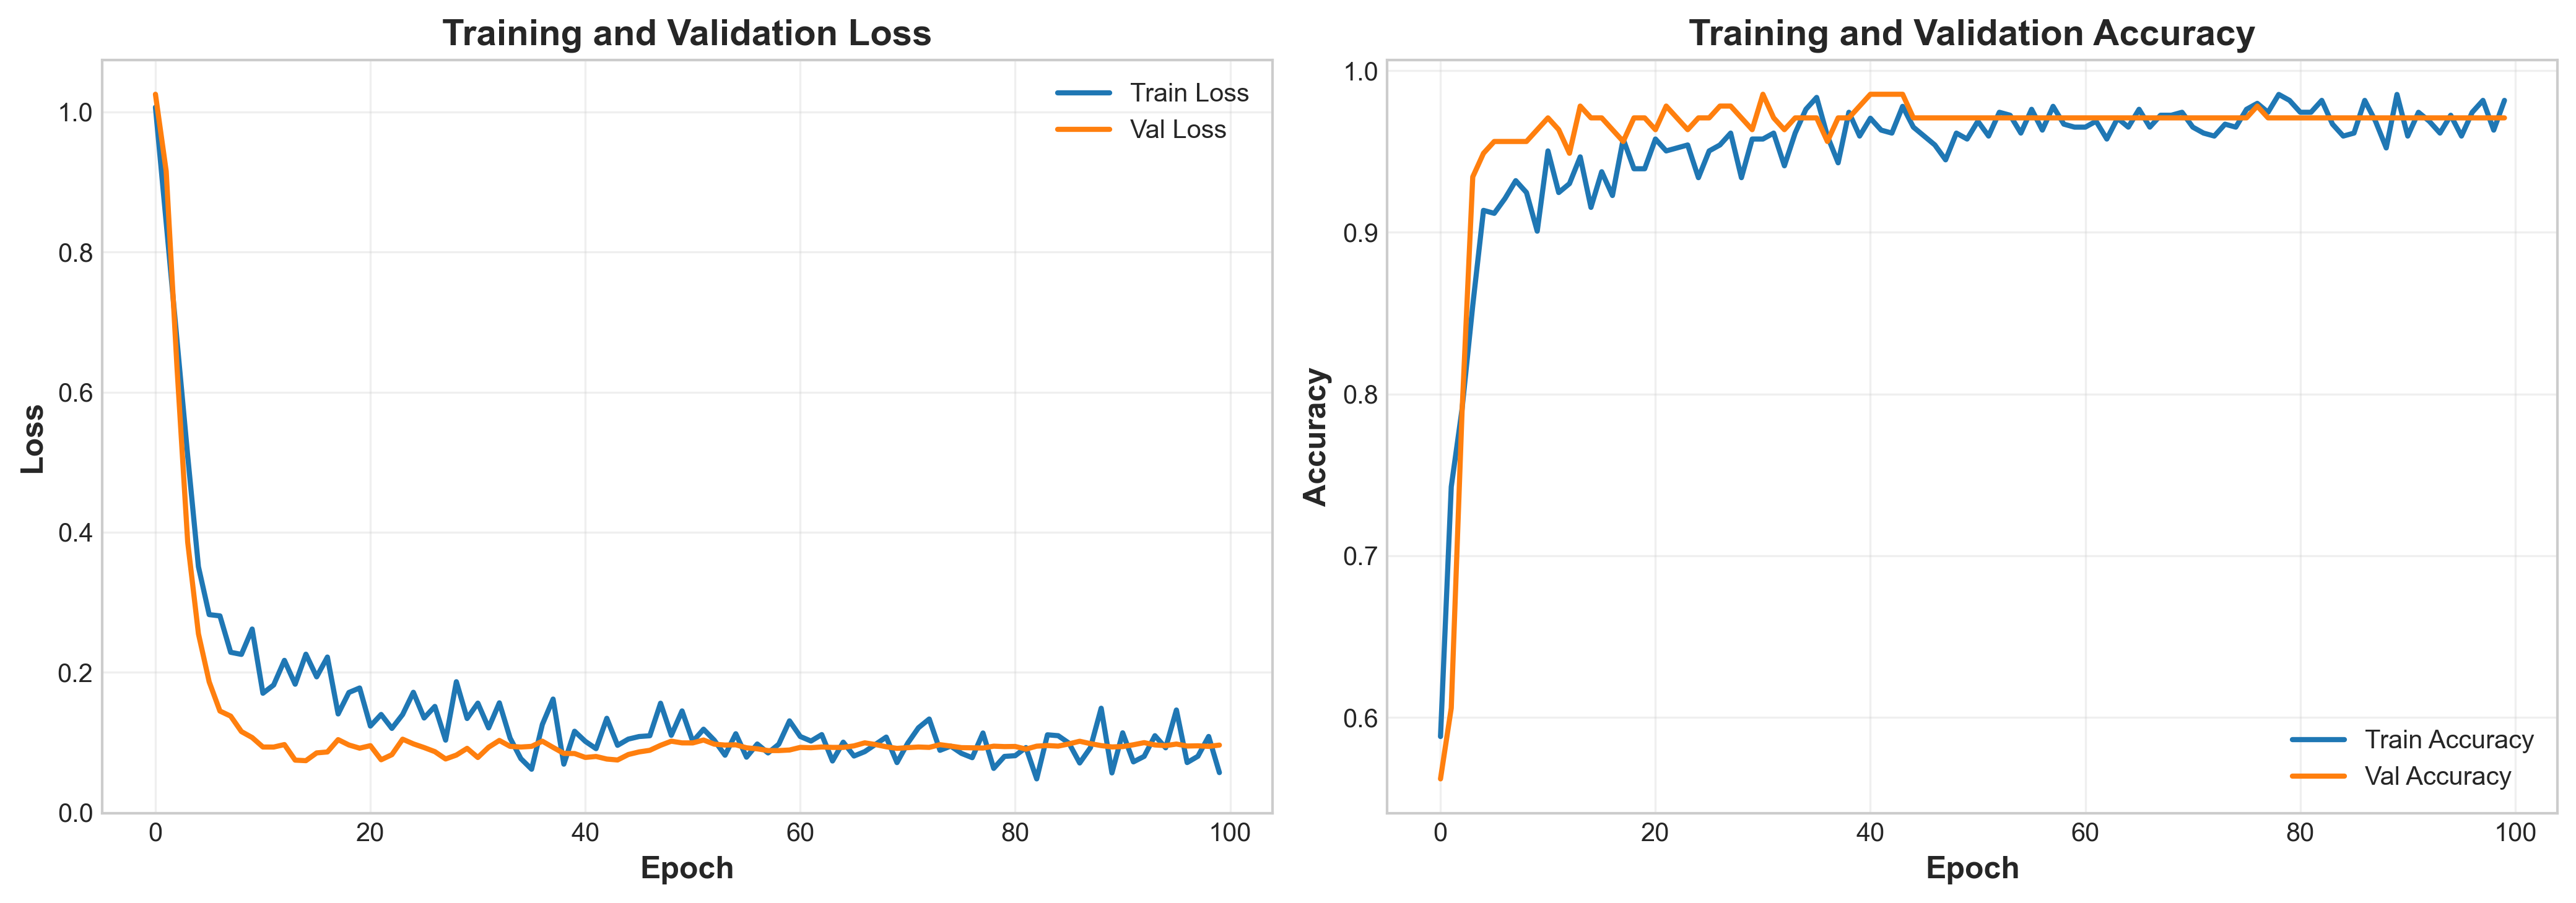
\includegraphics[width=\linewidth,height=1.05in,keepaspectratio]{figures/novel_deep_learning_training.png}
\caption{Deep learning model training dynamics for the attention-based neural network. Validation accuracy reached 97.1\%.}
\label{fig:dl_training}
\end{figure}


\subsection{Immune Cell Abundance and Network Dynamics}
Immune cell interaction network deviation from the normal reference was summarized using the immune cell interaction network disruption (ICIND) score.
Across tumor samples, the ICIND disruption score was 0.056 relative to the normal reference score of 0, indicating measurable divergence from the normal immune interaction architecture.
Phenotype-wise means of the dysregulation score are summarized in Table~\ref{tab:dysregulation_means}. Figure~\ref{fig:quantiseq_stacked} summarizes the quanTIseq-derived immune cell proportions by phenotype and provides visual context for the deconvolved cell-composition inputs used in the network-dynamics analysis.

\begin{table}[!t]
\centering
\caption{Mean dysregulation score by immune phenotype.}
\label{tab:dysregulation_means}
\begin{tabular}{lc}
\toprule
\textbf{Phenotype} & \textbf{Mean dysregulation score} \\
\midrule
Immune-Inflamed   & 3.00 \\
Immune-Suppressed & 3.88 \\
Immune-Desert     & 3.25 \\
\bottomrule
\end{tabular}
\end{table}

\begin{figure}[!t]
\centering
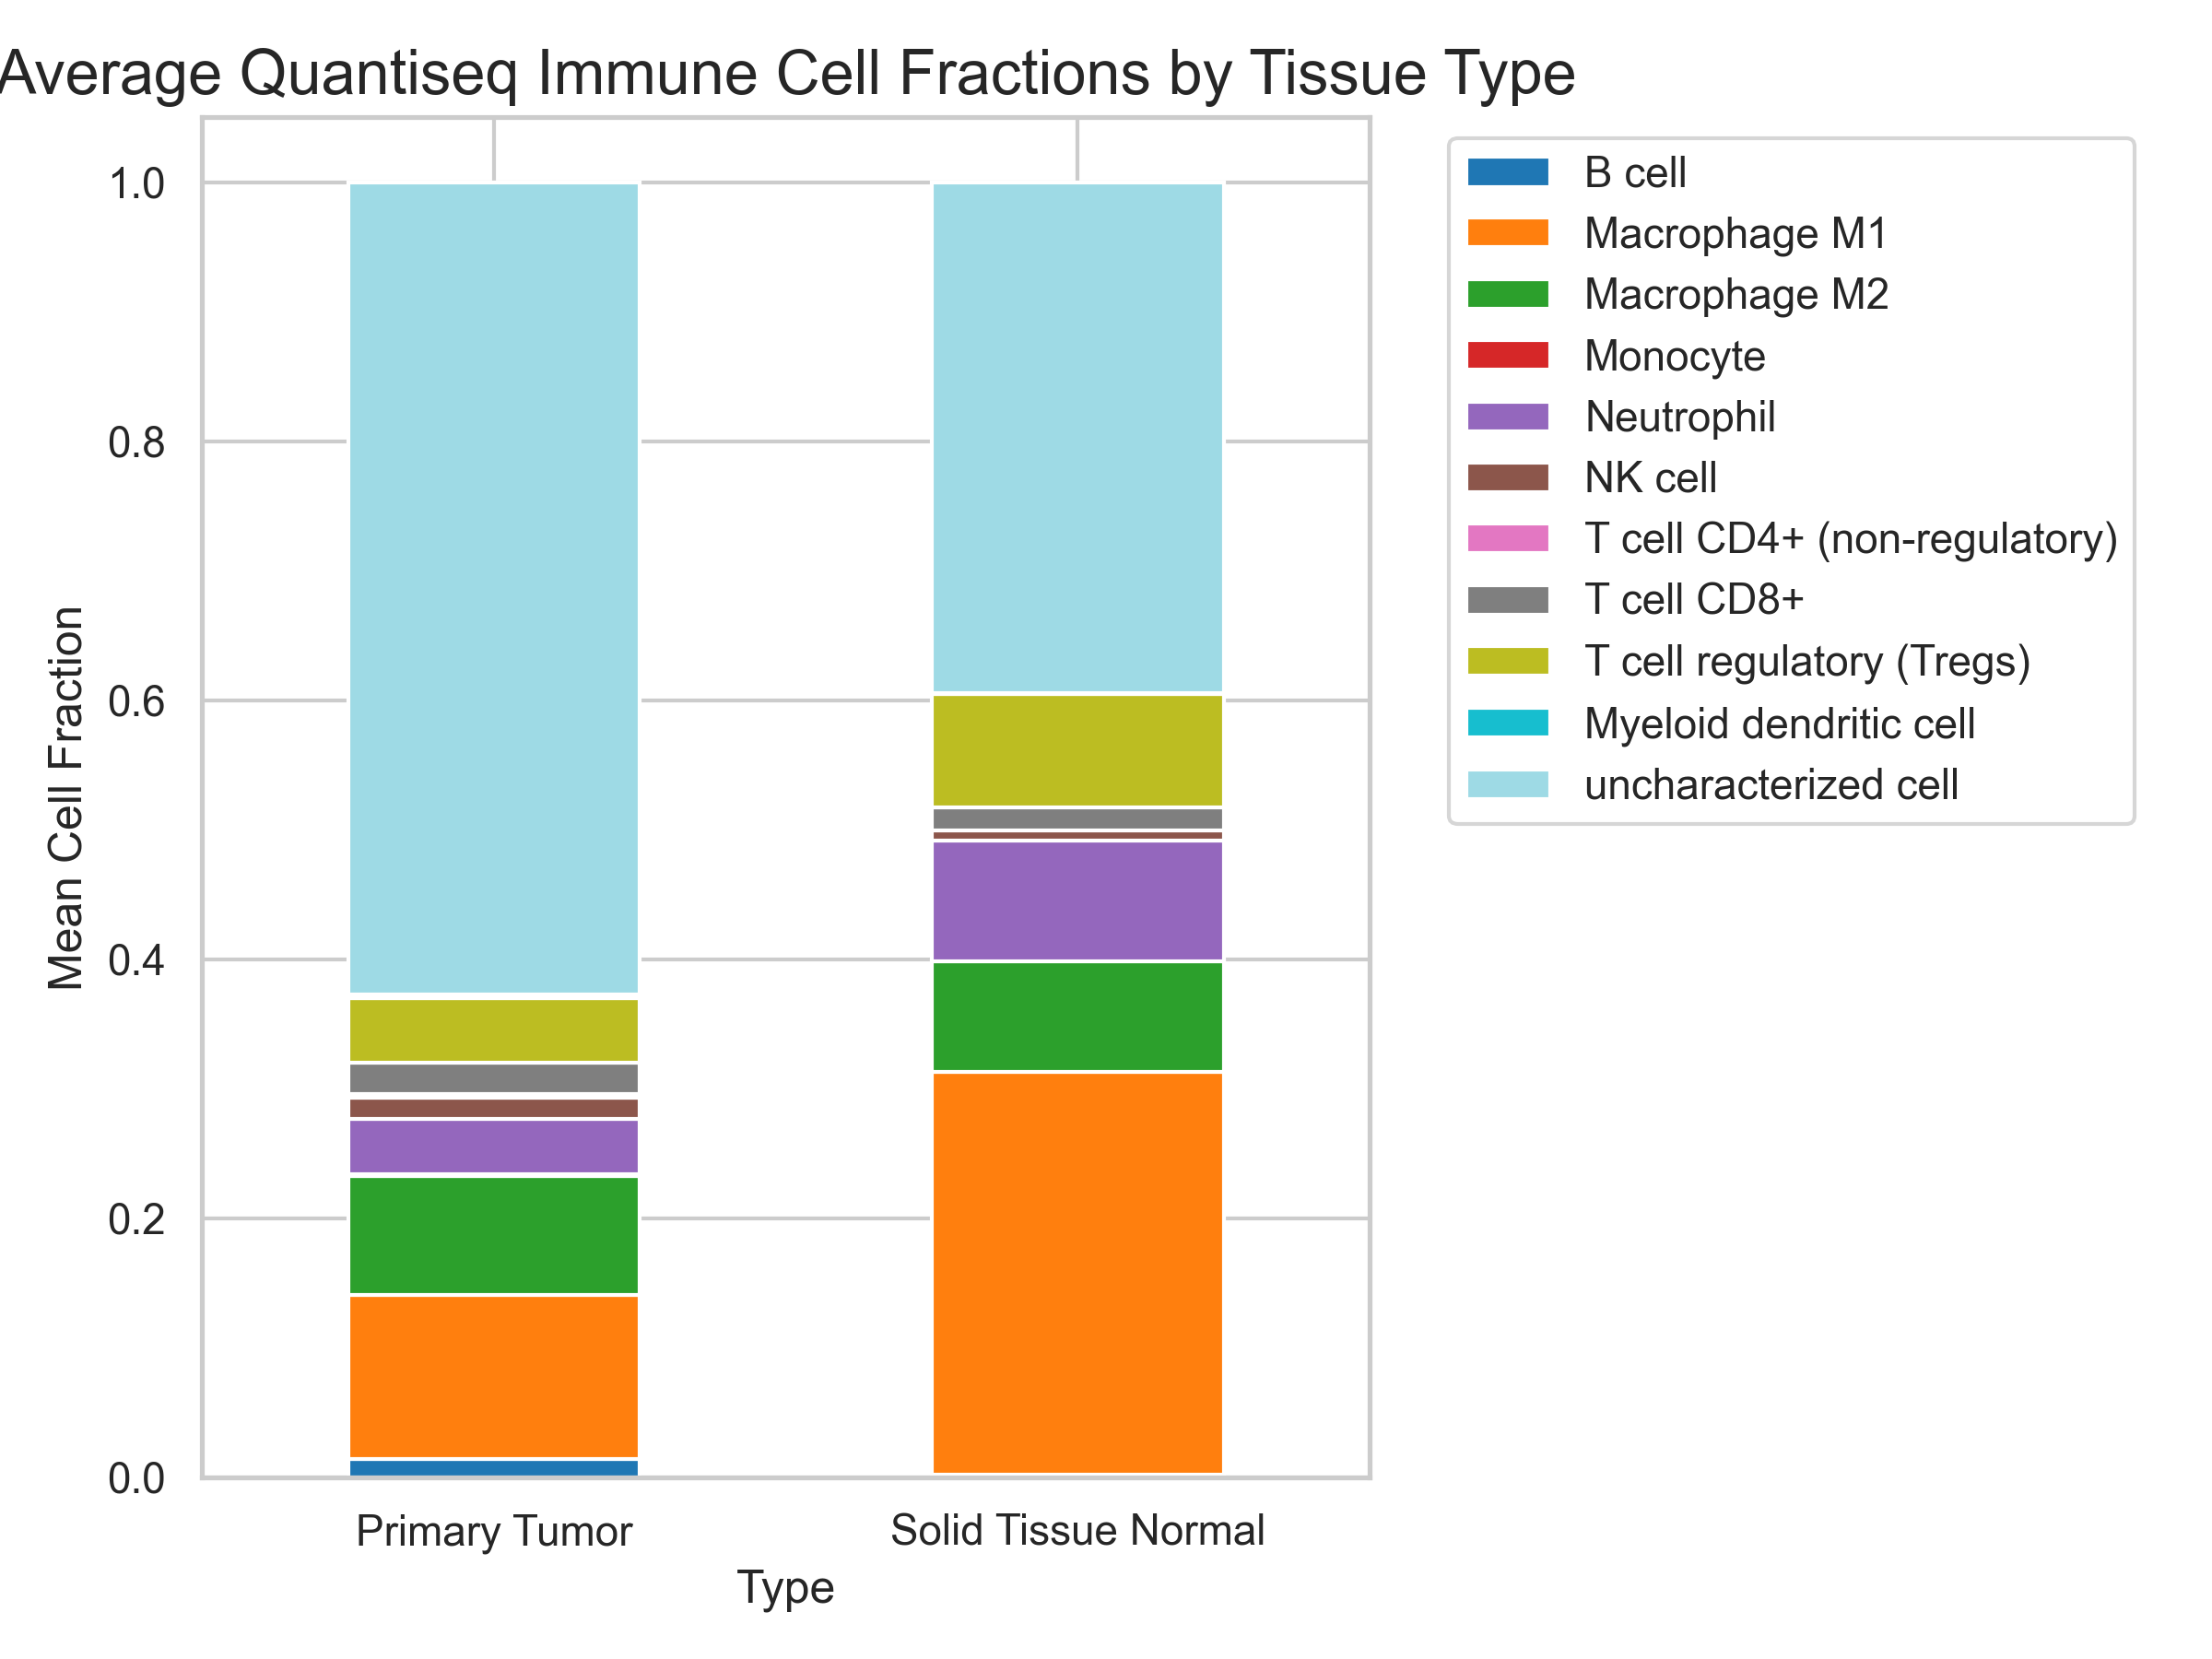
\includegraphics[width=\linewidth,height=1.45in,keepaspectratio]{figures/quantiseq_stacked_bar_aggregated.png}
\caption{quanTIseq stacked bar chart showing immune cell proportions across all TCGA-LUAD samples, grouped by immune phenotype.}
\label{fig:quantiseq_stacked}
\end{figure}








\section{Discussion}
\subsection{Summary of Key Findings}
This study analyzed 515 TCGA-LUAD bulk RNA-seq tumor profiles to derive immune landscape features, assign samples to immune phenotypes, and evaluate associations with overall survival.
The phenotype prediction model produced consistent phenotype assignments on the validation split, and survival curves differed across inferred immune phenotypes.
In addition, immune cell interaction network analysis yielded measurable deviations of tumor immune interaction structure from a normal reference network.

\subsection{Interpretation of Immune Phenotype Stratification}
The observed differences in phenotype-stratified Kaplan--Meier curves were consistent with the premise that TIME heterogeneity is reflected in bulk transcriptomic profiles and can be summarized into discrete immune states.
These results align with prior descriptions of recurrent immune ``states'' or immune contexture variation across tumors, in which immune activity and immunosuppression can co-occur and vary across patients \cite{Fridman2017,Thorsson2018,ChenMellman2017}.
Within this framework, phenotype labels provide a compact representation of immune landscape variation that can be used for downstream analyses of outcome heterogeneity.

\subsection{Relevance of Network-Level Immune Disruption}
Beyond marginal immune cell abundance, the network analysis emphasized coordination patterns among immune populations by quantifying deviations from a normal reference interaction structure.
A non-zero disruption score in tumors suggests that tumor-associated immune composition was accompanied by changes in inferred immune cell relationship patterns.
This system-level representation complements deconvolution-based estimates by capturing relationships among inferred cell types rather than treating each fraction as an independent covariate.

\subsection{Comparison With Existing Computational Immune Profiling Studies}
Prior work has established that bulk transcriptomes can be used to estimate immune and stromal composition using reference-based deconvolution and signature scoring approaches \cite{Newman2015,Finotello2019,Becht2016,Aran2017xCell,Sturm2019}.
The present study followed this general line of evidence by using deconvolution-derived immune landscape features as a substrate for phenotype assignment and outcome analysis.
The network-based representation extends common downstream workflows (e.g., comparing individual cell fractions) by summarizing coordinated immune structure in a form that can be integrated with phenotype labels.

\subsection{Limitations}
Several limitations should be considered.
First, bulk RNA-seq aggregates signals across diverse cell types and does not directly resolve spatial organization or cell-state specificity, which can be important for understanding TIME function \cite{Fridman2017,ChenMellman2017}.
Second, analyses were conducted on a retrospective cohort from TCGA, and clinical annotation granularity and treatment information are limited relative to prospective studies \cite{TCGA_LUAD_2014,Grossman2016GDC}.
Third, the phenotype model and survival associations were not evaluated on an independent external LUAD cohort, so generalizability across platforms and institutions remains to be established.


\subsection{Therapeutic Implications of Immune Phenotype Stratification}
The immune phenotype framework provides a basis for generating treatment hypotheses rather than clinical recommendations. Immune-Inflamed tumors were characterized by higher CD8$^+$ T-cell infiltration and TCR diversity, whereas Immune-Suppressed tumors showed higher estimated M2 macrophage and regulatory T-cell proportions; Immune-Desert tumors had generally low inferred immune infiltration. A computational perturbation that reduced M2 macrophage abundance by 50\% and increased CD8$^+$ T-cell abundance by 50\% changed the dysregulation score for Immune-Suppressed samples. Because this in silico perturbation does not estimate treatment response or causal effects, its interpretation is limited to hypothesis generation. Any phenotype-specific therapeutic strategy requires independent experimental and prospective clinical validation.

\subsection{Future Directions}
Future work should include validation on external cohorts with harmonized processing, sensitivity analyses across alternative deconvolution frameworks, and evaluation of phenotype stability across resampling and batch perturbations.
Where available, integrating orthogonal immune measurements (e.g., multiplex imaging or single-cell data) could support triangulation of phenotype definitions and network disruption metrics.
Finally, extending the modeling to incorporate additional covariates and standardized clinical endpoints may improve interpretability and facilitate comparison across studies.

\section{Conclusion}
This study developed an immune phenotyping and analysis pipeline for TCGA lung adenocarcinoma using bulk RNA-seq-derived immune landscape features. The resulting immune phenotypes were predicted with high validation performance (97.1\% accuracy using an attention-based deep learning model). Kaplan--Meier analysis across the three immune phenotypes yielded $p=0.0091$, supporting the hypothesis that immune microenvironment composition is associated with patient survival outcomes. The ICIND network disruption analysis revealed a measurable divergence (score $=0.056$) between tumor and normal immune interaction architecture, demonstrating the value of system-level immune modeling. This framework suggests that non-invasive, transcriptome-based immune profiling is a viable and scalable approach for characterizing tumor immune states in LUAD, with potential utility for informing immunotherapy patient selection and treatment planning.

\section*{Acknowledgment}
The authors acknowledge The Cancer Genome Atlas (TCGA) and the NCI Genomic Data Commons (GDC) for providing access to the molecular and clinical data used in this study. The authors also acknowledge the open-source software ecosystem that supports reproducible computational biology. This work was conducted independently as a student research project. No institutional affiliation is claimed for this work. Manuscript preparation was assisted by AI language model tools; all analyses, data, and scientific conclusions are the authors' own. Any opinions, findings, and conclusions are those of the authors and do not necessarily reflect the views of any institution.


\section*{Data Availability}
All TCGA-LUAD data used in this study are publicly available through the NCI Genomic Data Commons (\url{https://portal.gdc.cancer.gov/}). Clinical annotation data are available through the TCGA Clinical Data Resource. TCR sequencing summary statistics are available from published TCGA analysis files. Analysis code, processed result summaries, and manuscript source are available at \url{https://github.com/JayadityaVetsa/luad-immune-phenotyping}. A version-specific archival DOI will be added to the repository release metadata.

\bibliographystyle{IEEEtran}
\bibliography{references_real}

\end{document}
